\documentclass{standalone}
\usepackage{tikz}
\usepackage{helvet}
\renewcommand{\familydefault}{\sfdefault}
\usepackage{graphicx}
\graphicspath{
  {/home/sshin/git/shin-faculty-applications/},
  {/home/sshin/git/shin-faculty-applications/fig/},
  {/home/sshin/git/shin-faculty-applications/fig/old/},
  {/home/sshin/git/shin-faculty-applications/fig/nw-people/}
}
\begin{document}
\begin{tikzpicture}[align=center]
  \node (a) at (0,-.75) {};
  \foreach \x in {1,2,3,4}{
    \node (d\x) at (\x*2.5-2.5*2.5,-2.5) {};
    \node (dd\x) at (\x*2.5-2.5*2.5,-3) {};
    \node (e\x) at (\x*2.5-2.5*2.5,-5.5) {};
    \node[draw,lightgray] (f\x) at (\x*2.5-2.5*2.5,-7.25) {
      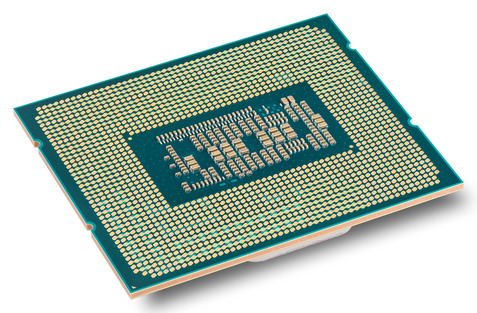
\includegraphics[height=20pt]{cpu.jpg}\\
      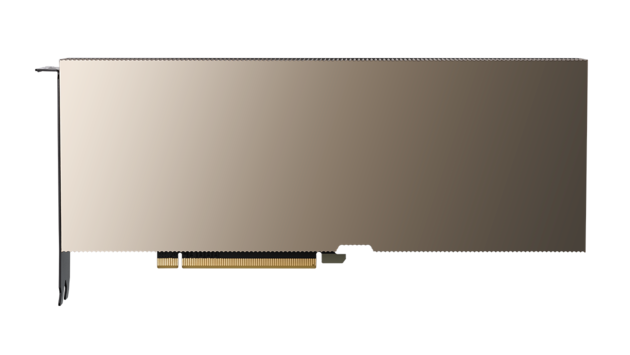
\includegraphics[height=20pt]{a100.png}
    };
    \draw[lightgray] (a.south) to (d\x.center);
    \draw[-latex,lightgray] (d\x.center) to (dd\x.center);
    \draw[-latex,lightgray] (e\x) -- (f\x);
  }
  \draw[latex-latex,lightgray] (f1.north) to [in=160,out=20] (f2.north);
  \draw[latex-latex,lightgray] (f2.north) to [in=160,out=20] (f3.north);
  \draw[latex-latex,lightgray] (f3.north) to [in=160,out=20] (f4.north);
  
  \node (c) at (0,-6) {Distributed Computing};
  \node at (a) {
    Full Problem\\
    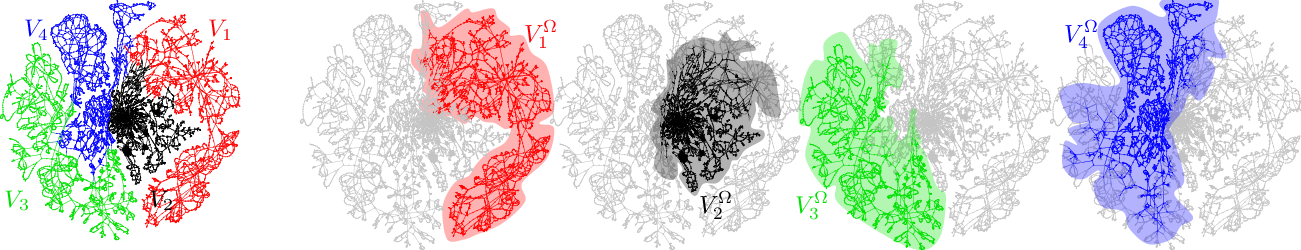
\includegraphics[scale=.4,trim={0 0 750 0},clip]{graph-abstract-old.png}
  };
  \node (b) at (0,-4) {
    Decomposition\\
    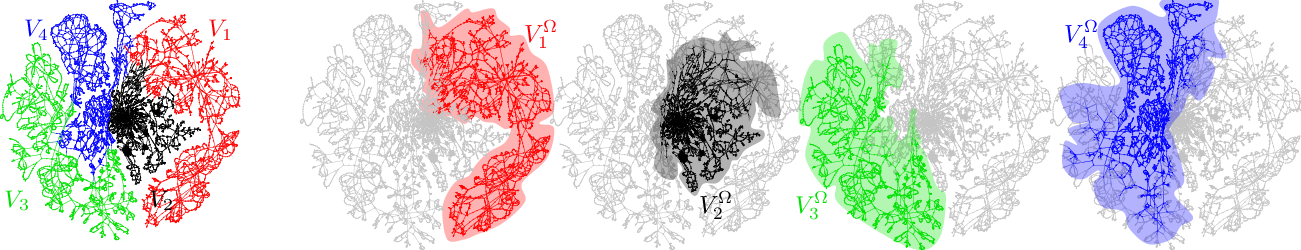
\includegraphics[scale=.4,trim={200 0 0 0},clip]{graph-abstract-old.png}
  };
  % \draw[-latex] (a) -- node[black] {} (b);
  % \node[font=\scriptsize] at (-5,0) {
  %   \begin{tikzpicture}
  %     \node at (0,0) {
  %       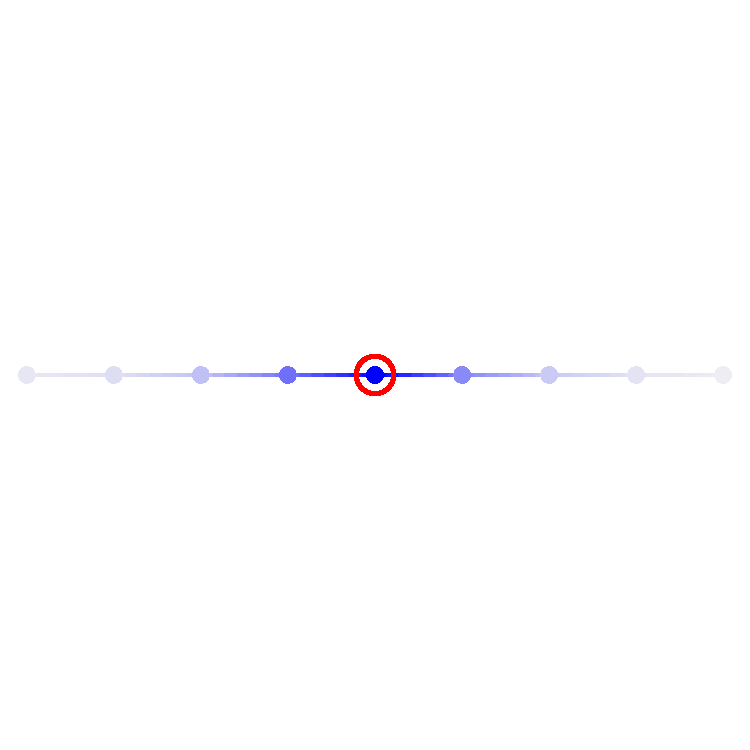
\includegraphics[width=.22\textwidth]{ocp-hm-1.pdf}
  %     };
  %   \end{tikzpicture}
  % };
  % \node[font=\scriptsize] at (-2,0) {
  %   \begin{tikzpicture}
  %     \node at (0,0) {
  %       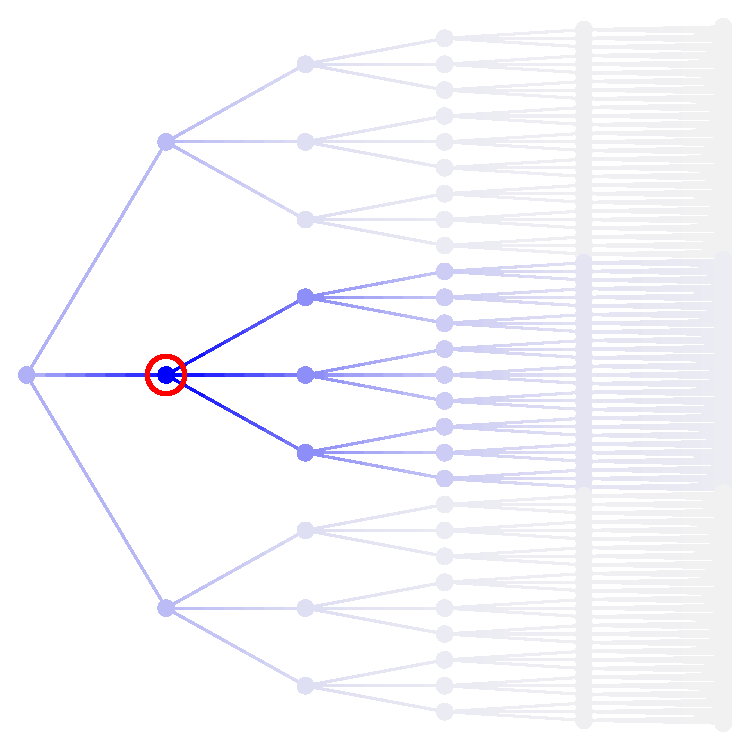
\includegraphics[width=.22\textwidth]{sto-hm-1.pdf}
  %     };
  %   \end{tikzpicture}
  % };
  % \node[font=\scriptsize] at (-5,-2.7) {
  %   \begin{tikzpicture}
  %     \node at (0,0) {
  %       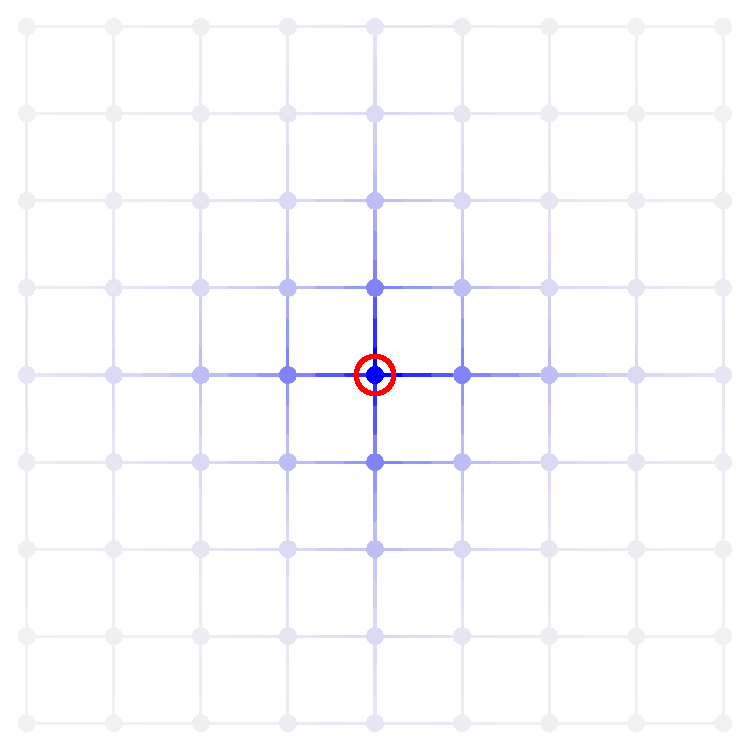
\includegraphics[width=.22\textwidth]{pde-hm-1.pdf}
  %     };
  %   \end{tikzpicture}
  % };
  % \node[font=\scriptsize] at (-2,-2.7) {
  %   \begin{tikzpicture}
  %     \node at (0,0) {
  %       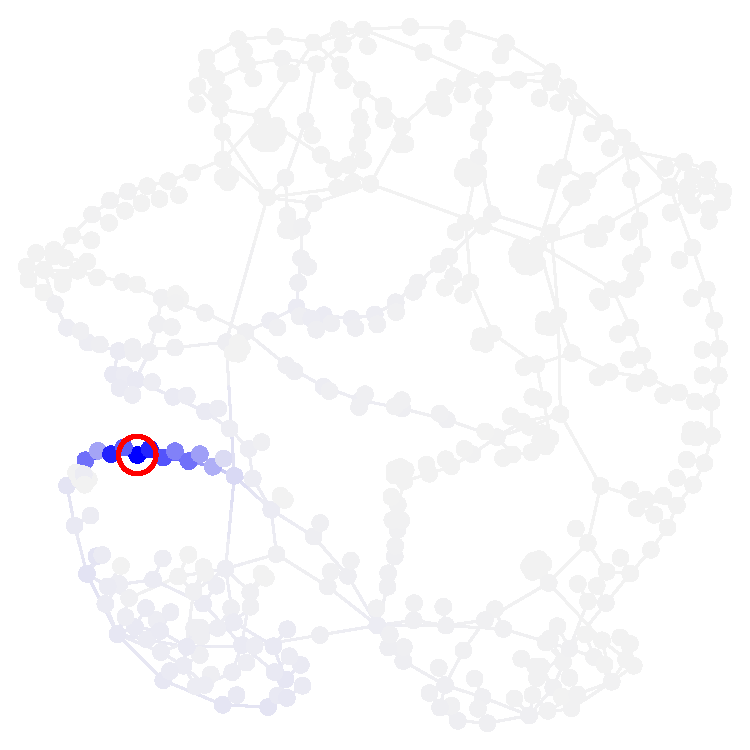
\includegraphics[width=.22\textwidth]{opf-hm-1.pdf}
  %     };
  %   \end{tikzpicture}
  % };
\end{tikzpicture}
\end{document}